\documentclass[12pt,openright,twoside]{report}
\usepackage[a4paper,top=25mm,bottom=25mm,right=25mm,left=25mm,bindingoffset=6mm]{geometry}
\usepackage[utf8]{inputenc}
\usepackage[swedish,british]{babel}
\usepackage{amsmath}
\usepackage{graphicx}
\usepackage{pict2e}
\usepackage{tabu}
\usepackage{booktabs}
\usepackage{bookmark,hyperref}
\usepackage{gensymb}
\graphicspath{{Bilder/}}

%Formatering av rubriker
%%%%%%%%%%%%%%%%%%%%%%%%%%%%%%%%%%%%%%%%%%%%%%%%%%%%%%%%%%%%%%%%%%%%%%%%%%%%%%%%%%%%%%%
\usepackage{titlesec, blindtext, color}
\titleformat{\chapter}[hang]{\Huge\bfseries}{\thechapter}{20pt}{}{}
\titlespacing*{\chapter}{0pt}{*0}{*3}
\titlespacing*{\section}{0pt}{*4}{*1}
\titlespacing*{\subsection}{0pt}{*3}{*0}
\titlespacing*{\subsubsection}{0pt}{*4}{*1}

\setcounter{secnumdepth}{2}
\setcounter{tocdepth}{2}
%%%%%%%%%%%%%%%%%%%%%%%%%%%%%%%%%%%%%%%%%%%%%%%%%%%%%%%%%%%%%%%%%%%%%%%%%%%%%%%%%%%%%%%

\usepackage{tocloft} %Control the ToC formatting

\setlength{\parindent}{0pt}
\setlength{\parskip}{1em}

%Formatering av sidornummer (Comment to have the number centered)
%%%%%%%%%%%%%%%%%%%%%%%%%%%%%%%%%%%%%%%%%%%%%%%%%%%%%%%%%%%%%%%%%%%%%%%%%%%%%%%%%%%%%%%
\usepackage{fancyhdr}
\pagestyle{fancyplain}%
\fancyhf{} % clear all header and footer fields
\fancyfoot[RO,LE]{\thepage}
\renewcommand{\headrulewidth}{0pt}
%%%%%%%%%%%%%%%%%%%%%%%%%%%%%%%%%%%%%%%%%%%%%%%%%%%%%%%%%%%%%%%%%%%%%%%%%%%%%%%%%%%%%%%

\usepackage[hang, font=small, labelfont=bf]{caption}
\usepackage{subcaption}
\captionsetup{justification   = raggedright,
              singlelinecheck = false,
              format = hang}

\usepackage[
  backend=bibtex,
  %%%%% For NameYear citation
  %   style=authoryear,
  %   citestyle=authoryear-comp,
  %   sorting=nyt
  %%%%%
  %%%%% For Number citation
  style=numeric,
  citestyle=numeric,
  sorting=none,
  %%%%%
  maxcitenames=2,maxbibnames=99,
  natbib]
{biblatex}
\addbibresource{Referenser.bib}


%%%%%%%%%%%%%%%%%%%%%%%%%%%%%%%%%%%%%%%%%%%
% DO NOT NEED TO CHANGE BEFORE THIS POINT %
%%%%%%%%%%%%%%%%%%%%%%%%%%%%%%%%%%%%%%%%%%%

\hypersetup{
    colorlinks=true,
    linkcolor=black,
    anchorcolor=black,
    citecolor=black,
    urlcolor=black,
    pdftitle={TITEL},  % Skriv din titel här
    pdfauthor={Författarens Namn}, % Skriv ditt namn här
    }

\title{
    {\LARGE TITEL}\\ % Skriv din titel här
    {\large UNDERTITEL}\\
    {\vspace{10mm}}
    {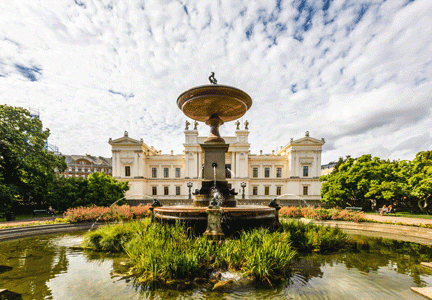
\includegraphics[width=0.6\textwidth]{Cover_Figure.png}}
    }
\author{Författarens Namn} % Skriv ditt namn här
\date{\today}

\begin{document}

\selectlanguage{swedish}
\maketitle
\clearpage

\thispagestyle{empty}
\mbox{}
\clearpage

\setcounter{page}{1}
\pagenumbering{Roman}

\chapter*{Abstract}
\addcontentsline{toc}{chapter}{Abstract}

\selectlanguage{british}

Add your abstract in english here

\selectlanguage{swedish}
\chapter*{Sammanfattning}
\addcontentsline{toc}{chapter}{Sammanfattning}

Skriv sammanfattning på svenska här
\chapter*{Förord}
\addcontentsline{toc}{chapter}{Förord}

Skriv ditt förord här

\selectlanguage{swedish}
\chapter*{Notation}
\addcontentsline{toc}{chapter}{Notation}

\subsection*{Latinska bokstäver}

$a$ - beskrivning\\
$b$ - beskrivning

\subsection*{Grekiska bokstäver}

$\alpha$ - beskrivning\\
$\beta$ - beskrivning


\cleardoublepage
\tableofcontents
\addcontentsline{toc}{chapter}{Innehåll}

\cleardoublepage
\setcounter{page}{1}
\pagenumbering{arabic}

\chapter{Titel på kapitel 1}

Skriv din text här

\section{Referenser}

Referens till en bok eller en artikel görs så här \citet{einstein1954ideas}, om författarnas namn är en del av texten, eller så här \citep{einstein1935can} om du hänvisar till publikationen indirekt.

\section{Ekvationer}

Ekvationer skrivs enligt följande

\begin{equation}
    E=mc^2
    \label{eq:energy}
\end{equation}

och refereras i texten så här \ref{eq:energy}.

\subsection{Tips för ekvationer}

På \href{http://www.codecogs.com/latex/eqneditor.php}{den här länken} kan du enkelt generera \ \LaTeX koden för dina ekvationer.

\subsubsection{Subsubsection titel}

Subsubsections har inga nummer och visas inte i innehållsförteckningen.
\chapter{Titel på kapitel 2}

\section{Bilder}

Bilder inkluderas enligt följande

\begin{figure}[h!] %the option h! forces the figure in this position
    \centering
    
\includegraphics{example_figure.jpeg}
    \caption{Skriv bildtexten här}
    \label{fig:example_figure}
\end{figure}

och refereras i texten så här: figur \ref{fig:example_figure}.
Spara alla bilder i mappen ``Bilder''.

\section{Tabeller}

Tabeller skapas enligt följande

\begin{table}[t]
\caption{Skriv tabelltexten här}. 
\label{tab:example_table}
\begin{tabu} to\linewidth{ X[2,l] | X[1,l] X[1,c] X[1,r] }
    \toprule 
    Kolumn 1 har dubbel bredd & Kolumn 2 är vänsterjusterad & Kolumn 3 är centrerad & Kolumn 4 är högerjusterad \\
    \midrule 
    Värde & Värde & Värde & Värde \\
    \hline
    Värde & Värde & Värde & Värde \\
    \hline
    Värde & Värde & Värde & Värde \\
    \hline
    Värde & \multicolumn3{l}{Så här skriver du på flera kolumner}\\
    \hline
    Värde & \multicolumn3{r}{och ändrar justering}\\
    \bottomrule
\end{tabu}
\end{table}

och refereras i texten så här: tabell \ref{tab:example_table}

\cleardoublepage
\addcontentsline{toc}{chapter}{Litteratur}
\printbibliography

\appendix
\titleformat{\chapter}[display]{\Huge\bfseries}{Bilaga \thechapter}{10pt}{}{}

\chapter{Titel Bilaga A}

Skiv din text här

\end{document}